% Define document class
\documentclass[twocolumn]{aastex63}
\DeclareRobustCommand{\Eqref}[1]{Eq.~\ref{#1}}
\DeclareRobustCommand{\Figref}[1]{Fig.~\ref{#1}}
\DeclareRobustCommand{\Tabref}[1]{Tab.~\ref{#1}}
\DeclareRobustCommand{\Secref}[1]{Sec.~\ref{#1}}
\newcommand{\todo}[1]{{\large $\blacksquare$~\textbf{\color{red}[#1]}}~$\blacksquare$}
\newcommand{\mr}[1]{{\textbf{\color{green!75!black}[#1]}}}
% \usepackage{cuted}
\usepackage{flushend}
\usepackage{amsmath}
% \graphicspath{{./figures/}}

\begin{document}

% Title
\title{On the prevalence of early mass transfer for very massive binaries}

\author[0009-0008-2061-4946]{C.~A.~Burt}
\affiliation{University of Arizona, Department of Astronomy \& Steward Observatory, 933 N.~Cherry Ave., Tucson, AZ 85721, USA}

\author[0000-0002-6718-9472]{M.~Renzo}
\affiliation{University of Arizona, Department of Astronomy \& Steward Observatory, 933 N.~Cherry Ave., Tucson, AZ 85721, USA}

\author[0000-0002-2215-1841]{A.~Grichener}
\affiliation{University of Arizona, Department of Astronomy \& Steward Observatory, 933 N.~Cherry Ave., Tucson, AZ 85721, USA}

\begin{abstract}
  Common phases of mass transfer in stellar binaries are case A
  (during the donor's main sequence) and case B (after the donor's
  main sequence but before helium core depletion). For most masses,
  radii significantly grow after the main sequence, making case B more
  common. However, depending on uncertain stellar physics, very
  massive stars may already undergo significant expansion during the
  main sequence increasing the probability of case A mass transfer.
  For observationally-informed convective boundary mixing, case A mass
  transfer dominates for donor masses $\gtrsim 75 \, M_{\odot}$. This
  is not the case without convective boundary mixing or in the stellar
  models commonly used in rapid binary population synthesis.
  Therefore, case A mass transfer may be more dominant than commonly
  assumed, with potential impact on rates of all post mass transfer
  binaries, from Wolf-rayet-O-type binaries, to X-ray binaries, and
  gravitational wave progenitors.
\end{abstract}

\section{Mass Transfer in Very Massive Binaries}

Binary stars with a sufficiently small orbital separation
($a\lesssim2500\,R_{\odot}$) undergo (at least) a mass transfer phase
in which the donor star transfers mass the initially less massive
accretor. For very massive stars ($ \gtrsim 30 \, M_{\odot}$), mass
transfer most often occurs during the donor's hydrogen core-burning
main sequence (case A) or helium core-burning (case B), which together cover
$\sim99\%$ of the donor's lifetime \citep{kippenhahn:67}.

\begin{figure*}[htbp]
  \centering
  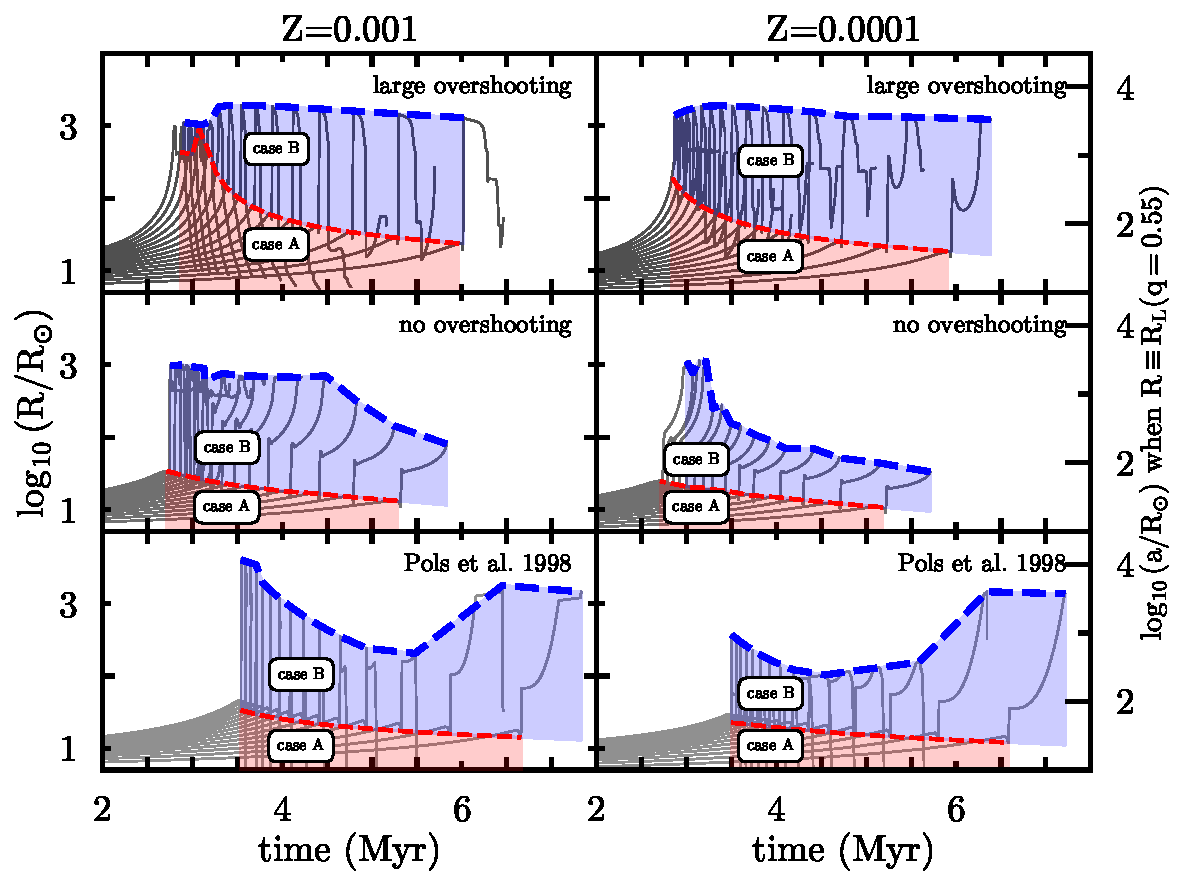
\includegraphics[width=0.9\textwidth]{radii}
  \caption{Each panel contain 15 stellar models spanning from a
    $30 \, M_{\odot}$ star on the right to a $100 \, M_{\odot}$ with
    intervals of width $5 \, M_{\odot}$. The top panels plot models
    that feature broad convective boundary mixing, the middle panels
    plot models that do not feature overshooting, and the bottom
    panels plot models generated from COMPAS using data from
    \cite{pols:98}. The left panels have a metallicity $Z=0.001$ and
    the right panels have a metallicity $Z=0.0001$}
  \label{fig:radii}
\end{figure*}


For a flat in $\log_{10}(a)$ initial initial separation distribution
\citep{opik:24}, case B is expected more often than case A mass
transfer, since most stars expand dramatically post-main sequence
\citep{vandenheuvel:69}. However, very massive stars may already
undergo a drastic expansion in radius during their main sequence.
\citep[e.g.,][]{sanyal:15, jiang:15, sabhahit:24}. This may increase
the rate of case A \citep{demink:08}, which could have significant
implications on the rates of Wolf-Rayet+O-type binaries
\citep[e.g.,][]{nuijten:24}, X-ray binaries, and gravitational wave
progenitors. The radius of the donor is dependent on unknown stellar
parameters, including stellar winds \citep{renzo:17, josiek:24},
metallicity \citep{xin:22}, close-to-super-Eddington-layers
\citep[e.g.,][]{joss:73, paxton:13, jiang:15, agrawal:22, jermyn:23},
and convective boundary mixing \citep{anders:23, johnston:24}. Here,
we illustrate this comparing the radial evolution of very massive
stars varying convective boundary mixing, metallicity, and models
commonly adopted in rapid binary population synthesis.

\section{Comparing Donor Radii}

We computed \textsc{MESA} models (version 24.03.1, \citealt{paxton:11,
  paxton:13, paxton:15, paxton:18, paxton:19, jermyn:23}) from
$30 \, M_{\odot}$ to $100 \, M_{\odot}$ in steps of $5\,M_\odot$ at
metallicity $Z=0.001$ and $0.0001$ following the setup from
\cite{renzo:23}. The gray lines in \Figref{fig:radii} show their
radial evolution as a function of time.

We explore models with (top panel) and without overshooting (middle
panel) and compared them to the \cite{pols:98} models (bottom panel)
used in \textsc{SSE/BSE} \citep{hurley:00} taken from \textsc{COMPAS}
\citep{stevenson:17, vignagomez:18, riley:22}, which extrapolates for
masses $\geq50\,M_\odot$.

When using overshooting, our \textsc{MESA} models implement an
exponential algorithm \citep{herwig:00} fit to the step overshooting
calibrated on the width of main sequence in 30 Doradus
\citep{brott:11} following \cite{claret:18}. This relatively ``large
overshooting'' model is compared to models not including any
convective boundary mixing, and to the \cite{pols:98} models including
an effectively mass-dependent overshooting.

The red and blue dashed lines in each panel of \Figref{fig:radii}
denote the maximum radius during the main sequence and helium core
burning phase, respectively. These mark the maximum Roche radius for a
case A and case B donor, respectively. The right axis shows orbital
separations $a$ where the stellar radius meets the roche radius
\citep{eggleton:83}, neglecting orbital widening due to winds
(included in the stellar models) and assuming a representative
accretor-to-donor mass ratio of $q=0.55$. The red regions denote
binaries which will undergo case A mass transfer and the blue regions
denote binaries which will undergo case B mass transfer.

For $Z=0.001$, when including overshooting (top left panel), donors
with masses $ \gtrsim 75 \, M_{\odot}$ can only experience case A.
Removing convective boundary mixing (middle) keeps main sequence radii
smaller, preserving the blue region above the red line for case B mass
transfer at all masses. The overshooting implementation from
\cite{pols:98} (bottom), while nonzero, still leaves a large window
for case B up to $100 \, M_{\odot}$. At even lower metallicities of
$Z=0.0001$ (right), stars are more compact, and all models allow for
case B mass transfer at all masses.

\section{Implications for Post-Mass-Transfer Binaries}

Convective boundary mixing \citep{brott:11, johnston:24} and
metallicity have a strong effect on stellar radii, which determine
when a donor fills its Roche lobe. Other effects on stellar radii have
been explored elsewhere, including the adopted wind mass loss rates
\citep[e.g.,][]{smith:14, renzo:17, josiek:24}, rotation (and
consequently tides, e.g., \citealt{maeder:00}), and the treatment of energy transport
in correspondende of opacity bumps in the envelope
\citep[e.g.,][]{joss:73, agrawal:22, cheng:24}.

After a thermal-timescale initial phase, Case A mass transfer occurs
overall on a longer (nuclear) timescale, while case B occurs entirely
on a much shorter (thermal) timescale \citep[but see][]{klencki:22}.
Moreover, the dynamical stability of the orbit during mass transfer is
sensitive to the evolutionary phase of the stars involved
\citep[e.g.,][]{claeys:14}. Therefore, whether a given binary
experiences a common envelope depends on more than just the mass
ratio. Here, we show the depence on donor mass, metallicity, and
convective boundary mixing. Comparing rows in \Figref{fig:radii} shows
that the stellar evolution models commonly used in rapid population
synthesis are qualitatively similar to our no overshooting models, in
the sense that they allow for case B mass transfer up to inital masses
of $100 \, M_{\odot}$ for metallicities relevant to galactic and
gravitational astronomy.

Given the critial role of mass transfer for the formation of many
binaries of interest, the fraction of systems experiencing case A in
respect to case B may significany impact predicted rates for post mass
transfer binaries, including Wolf-Rayet+O-type binaries, X-ray
binaries, and gravitational wave progenitors. In particular, the role
of the stable mass transfer channel \citep[e.g.,][]{marchant:21,
  vanson:22} for binary black hole mergers is currently hotly debated.
Our results highlight that stellar uncertainties influence the mode of
mass transfer and consequently the outcomes.


\bibliography{./donorR.bib}
\end{document}

%%% Local Variables:
%%% mode: latex
%%% TeX-master: t
%%% End:
